\section{Introduction}

Parallel patterns are a well established high-level parallel programming model for producing portable, maintainable, adaptive and efficient parallel code. They have been endorsed by some of the biggest IT companies, such as Intel and Microsoft, who have developed their own parallel pattern libraries (Intel TBB, Microsoft PPL etc.) A standard way of using these libraries is to start with the sequential code, identify in it the portions of the code that are amenable to parallelisation together with the exact parallel pattern to be applied, and then instantiating the identified pattern at the identified location in the code, after possibly restructuring the code to accommodate for parallelism. Sequential code gives the cleanest starting point for introduction of parallel patterns. There exists, however, a large base of \emph{legacy} code that was parallelised using lower-level, mostly ad-hoc parallelisation methods and libraries, such as \emph{pthreads}. This code is usually tailored to a specific parallelisation, all but preventing exploration of alternative parallelisation methods, and optimised for a specific system architecture. All this significantly reduces maintainability and portability of the code. %with highly-specific and tuned data structures which prevent alternative (possibly more efficient parallelisations) or portability to different platforms. Also, code maintainance requires intricate knowledge about the system architecture and various low-level underlying mechanisms such as thread creation, synchronisation and scheduling. 
Introducing pattern parallelism into legacy-parallel code would significantly improve the code quality, but this is usually a daunting task due to various factors, such as high degree of specialisation and custom tuning of the legacy code, incompability between \lstinline{pThreads} and parallel pattern libraries, usage of very specific, custom-built data structures tailored to a specific parallelism model etc.
  
This paper presents a \emph{software restoration} methodology for restructuring and refactoring legacy-parallel code. The overall process starts with an ad-hoc paralell code written using \lstinline{pThreads} or similar low-level library and, in the end, produces equivalent structured, pattern-based parallel programs. Our overall goal is to provide semi-automatic mechanisms based on software refactoring to guide the programmer through all stages of the process, suggesting source-to-source transformations and then, based on the programmer's input, automatically applying them. In this paper, we focus on the first stage of the methodlogy, namely \emph{parallelism elimination}, presenting refactorings to eliminate parallelism from legacy-parallel code, effectively transforming an application into the equivalent sequential version, with possibly some necessary concurrency still remaining in the code. We then demonstrate how manual application of the remaining steps of the methodolgy can produce semantically equivalent code that is comparable to the original legacy-parallel version in terms of execution speed, while significantly increasing portability, adaptivity and maintainability.

This paper, thus, makes the following specific research contributions:
\begin{itemize}
    \item We present the novel software restoration methodology for converting legacy-parallel applications into their structured parallel equivalents;
    \item We describe refactorings to eliminate parallelism from the legacy-parallel \lstinline{pthreads} code, providing semi-automatic implementation of the first step of software restoration methodology;
    \item We evaluate these refactorings on a set of benchmarks, demonstrating that removal of parallelism can allow us to manually derive the structured parallel code that is comparable to the original legacy-parallel version in terms of performance, while being more portable, adaptive and maintainable.
\end{itemize}

\section{Background}
Legacy-parallel code, written in ad-hoc way using low level parallel libraries such as \emph{pthreads}, is still very much present in various software repositories and projects. This code was usually developed by parallelism experts before the libraries and programming models for structured parallelisation became popular. It is usually tailored to one specific target machine and architecture, and might use highly-customised parallelisation and associated data structures. This makes it very hard to maintain that code, an increasing important feature in software engineering, or to port it to new architectures. It would be ideal if we could transform every legacy-parallel application into a structured parallel programs, written using high-level parallel programming libraries. However, for this to be possible, it is necessary that a well-defined underlying pattern of parallelism actually exists in the code, which can be exploited by instances of patterns. This is not always the case. However, in substantial number of cases, the parallelism in the application is an instance of one of the common patterns, such as farm, pipeline, workpool or stencil. In these cases, it should be possible, automatically or semi-automatically, to \emph{replace} unstructured parallelism with its structured (patterned) equivalent.   

\subsubsection*{Parallel Patterns}
%\begin{itemize}
%\item What are parallel patterns
%\item Some common patterns
%  \item Benefits of using patterns
%  \item Relevant pattern libraries (Open MP, Intel TBB...)
%\end{itemize}



\noindent
\emph{Parallel patterns} are a high-level abstraction for representing classes of computations that are similar in terms of their parallel structure, but different in terms of problem-specific operations. A typical example of a parallel pattern is a \emph{parallel map}, where the same operation is applied to a set of independent inputs in parallel. Regardless of whether the actual operation is, for example, multiplying a matrix by a vector, processing a pixel of an image or XX, the parallel structure of the computation will be the same. Parallel Patterns are typically implemented as library functions which handle creation, synchronisation and communication between the parallel threads, while the problem-specific (often sequential) computations are provided as the pattern parameters. In this paper, we restrict ourselves to two classical parallel patterns, which we believe to be the most common. Note that the technique described in this paper can be further generalised to include the full tractable set of parallel patterns.
\begin{itemize}
    \item The farm pattern models a data parallel computation, where a single computational worker, $f$, is applied to a set of independent inputs, $x_{1}, ..., x_{n}$. The parallelism arises from applying the worker, $f$, to different input elements at the same time in parallel. 
    \item The pipeline pattern models a parallel pipeline. Here, a sequence of functions, $f_{1}, f_{2}, ..., f_{m}$ are applied, to a stream on independent inputs, $x_{1}, ..., x_{n}$. The output of $f_{i}$ becomes the input to $f_{i+1}$, so that the parallelism arises from executing $f_{i+1}(f_{i}(...f_{1}(x_{k})...))$ in parallel with $f_{i}(f_{i-1}(...f_{1}(x_{k+1})...))$.
\end{itemize}

The benefits of using parallel patterns lie in clear separation between sequential and parallel parts of the code and high-level description of the underlying parallelism, which makes the patterned applications much easier to maintain, change and adapt to new architectures. For these reasons, they have been endorsed by most of the top IT companies, who have their own pattern libraries, such as Microsoft PPL~\cite{ppl} and Intel Thread Building Blocks~\cite{tbb}. In addition to that, there are also many popular open-source pattern libraries, such as OpenMP~\cite{openmp} and FastFlow~\cite{openmp}.

\subsubsection*{Software Refactoring}

\noindent
\emph{Software refactoring} is the process of changing the structure of a program while preserving
its functional semantics in order, for example, to increase code quality, programming
productivity and code reuse. In our case, refactorings are source-to-source transformations of the code that are performed \emph{semi-automatically}, under the programmers guidance and possibly with his input. In our previous work, we pioneered refactoring to introduce parallelism~\cite{rpl}, where sequential code is transformed to introduce instances of parallel patterns. We have shown that this can lead to excellent speedups of the resulting code.

\subsubsection*{Static and Dynamic Analysis}
\begin{itemize}
\item Mostly about analysis for pattern discovery, maybe we can lift from Adam's thesis
\end{itemize}

\section{Software Restoration}
\noindent
\emph{Software restoration} is a methodology based on refactoring and code analysis that aims to:
\begin{itemize}
\item \emph{discover} the instances of common patterns in legacy-parallel code;
\item \emph{eliminate} the \emph{undesirable} parallelism from the same code;
\item \emph{replace} the removed parallelism with instances of the parallel patterns;
\end{itemize}
The software restoration process takes as an input a legacy-parallel code, for which we currently assume it is written using the \emph{pthreads} library. It then applies a series of incremental program analysis and transformation steps, as depcited in the Figure~\ref{fig:SoftRest}, with the final result being an application based on parallel patterns that is semantically equivalent to the original legacy-parallel version. The software restoration involves the following steps:

\begin{figure*}
\centering
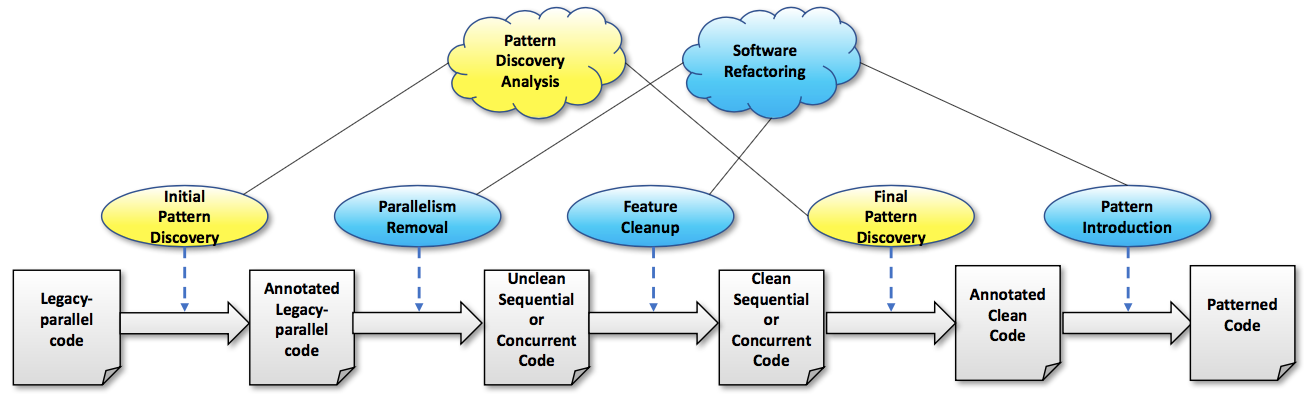
\includegraphics[width=\textwidth]{images/SoftRest.png}
\caption{Software Restoration Process}
\label{fig:SoftRest}
\end{figure*}

\begin{itemize}
\item \emph{Initial Pattern Discovery.} The initial program analysis step, applied to a legacy-parallel code, discovers i) parts of the threaded code that correspond to instances of parallel patterns; and, ii) parts of the threaded code that represent concurrent computations. Concurrent computations are, for example, separate threads that process the signals received by the user. It is necessary to know which threaded code is concurrent, as sequentialising these portions of code in the next step of the methodlogy can lead to deadlocks. Initial pattern discovery also annotates the legacy-parallel code, denoting the composition of patterns discovered, as well as the components of the pattern. Below is a part of the code for the legacy-parallel version of Matrix Multiplication example.

\begin{lstlisting}
static void *func (void* arg)
{
  data *input = (data *)arg;
  for (int i = input->start; i < input->end; i++) {
	  multiply_row_by_matrix(a, i, b, res);
  }
  return (void *)0;
}


void threads_create()
{
  pthread_attr_t attr;
  int status;
  int count=0;
  
  in = (data *) malloc (sizeof(data) * tc);
  thrs = (pthread_t *) malloc (sizeof(pthread_t) * tc);
  
  status = pthread_attr_init(&attr);
  if (status != 0)
    handle_error("Attribute initialisation failed!");

  #pragma farm(func,tc)   
  for (int tid=0; tid<tc; tid++) {  
    in[tid].start = count;
    in[thread_ind].row_end = count + chunk;
    count += chunk;

    status = pthread_create(&thr[tid], &attr,
                            &func, &in[tid]);
    if (status != 0)
      handle_error("Creating thread failed!");
  }
}

\end{lstlisting}

The pragma at the line 24 annotates the for loop as an instance of the \emph{farm} pattern, with \lstinline{func} being the farm worker function and \lstline{tc} being the number of workers (threads) in the farm.

\item \emph{Parallelism Removal.} In this first code transformation phase, we remove parts of the threaded code that are safe to remove (that is, all parallel parts except the parts identified as concurrent computations during the initial pattern discovery), and replace them with their sequential equivalents. This includes the calls to \emph{pthreads} functions for thread creation, synchronisation, mutex management and so on. This results in a sequential code that is semantically equivalent to the legacy-parallel version, but without parallelism (apart from possible concurrency constructs that are necessery for proper termination of the application). In the case of Matrix Multiplication, the code, after the parallelism removal, has the following form

\begin{lstlisting}
static void *func (void* arg)
{
  data *input = (data *)arg;
  for (int i = input->start; i < input->end; i++) {
	  multiply_row_by_matrix(a, i, b, res);
  }
  return (void *)0;
}


void threads_create()
{

  int status;
  int count=0;
  
  in = (data *) malloc (sizeof(data) * tc);

  




  #pragma farm(func,tc)   
  for (int tid=0; tid<tc; tid++) {  
    in[tid].start = count;
    in[thread_ind].row_end = count + chunk;
    count += chunk;

    func(&in[tid]);



  }
}
\end{lstlisting}

Note that all the \emph{pthread} constructs, together with the associated variables (\lstinline{status} and \lstinline{ths}) are removed, and the \lstinline{pthread_create} construct is replaced with the sequential call to the underlying thread function, \lstinline{func}. This is done with the help of the \lstinline{#pragma} annotation introduced by the initial pattern discovery, which tells us what kind of the pattern is there in the code (which, in turn, drives the refactoring decisions) and what is the farm worker function.

\item \emph{Feature Cleanup.} After the application of parallelism removal transformations, some artifacts of the legacy parallelisation may still remain in the code. These can be, for example, queues between stages of the pipeline computation or custom-build representations of flat data structures, such as arrays. These artifacts do not prevent the sequential version of application from running, but are redundant and might actually hinder alternative (and possibly better) parallelisations of the code. The next step is, therefore, to eliminate these artifacts and restore the code in the state as close to the original sequential code from which legacy parallelisation was derived as is poossible. This is, again, done using refactorings. As we are focusing on the \emph{farm} and \emph{pipeline} parallelism, the transformations we do is removing the queues of the pipeline stages (for the \emph{pipeline} parallelism) and flattening of data structures (in the case of \emph{farm} parallelism). The Matrix Multiplication code after feature cleanup is given below

\begin{lstlisting}
static void *func (void* arg)
{
  data *input = (data *)arg;
  for (int i = input->start; i < input->end; i++) {
	  multiply_row_by_matrix(a, i, b, res);
  }
  return (void *)0;
}


void threads_create()
{

  int status;
  int count=0;
  
  in = (data *) malloc (sizeof(data) * tc);

  




  #pragma farm(func,tc)   
  for (int tid=0; tid<tc; tid++) {  
    in[tid].start = count;
    in[thread_ind].row_end = count + chunk;
    count += chunk;

    func(&in[tid]);



  }
}
\end{lstlisting}
The array \lst{in} in the Matrix Multiplication code represented a block view of the flat array of indices of the matrix rows, which was introduced for the purpose of chunking to increase parallelism granularity in the legacy parallelisation based on the \emph{farm} parallelism. The array of all the rows of matrix \lstinline{b} was divided in as many chuncks as there are threads (\lstinline{tc}) and a chunk of this array assigned to each thread. Since modern pattern libraries, such as \emph{OpenMP} and \emph{TBB} can do chunking implicitly and dynamically, based on e.g.~the current system load, there is no need for explicit chunking to remain in the sequential code, even if it is going to be turned into patterned code again. Therefore, we eliminate the array \lstinline{in} and change the loop on line XX to iterate over the array of matrix rows instead.  
  
\item \emph{Additional Pattern Discovery.} Finally, once the code is restored into the state that is as close to the original sequential version as possible, further pattern discovery analysis can be made on it, as the feature cleanup transformations, and especially flattening of data structures and elimination of intermediate buffers/queues, might result in the code that has additional instances of parallel patterns that were not detected on the original, legacy-parallel code. This might enable us to parallelise the code in a different way than it was done in the original, legacy-parallel version, bringing possible benefits even in terms of performance.

\item \emph{Pattern Introduction.} After the final pattern discovery analysis is performed and the final patterns to be introduced are identified, together with the locations in the code where this will be done, the final step is to introduce instances of parallel patterns into the now-clean sequential code. This is again done using the software refactoring technology, where parts of the sequential code are replaced by calls to the functions from the high-level pattern libraries such as \lstinline{Intel TBB} or \lstinline{OpenMP}. This results in final, patterned parallel code that is semantically equivalent to the starting legacy-parallel code, but with much cleaner structure and simpler, higher-level code that allows easier maintainability, adaptivity and portability.
\end{itemize}

\section{Refactorings to Eliminate Parallelism} (2 pages)

\subsection{Replace \lstinline|pthread_create| with a function call}

This refactoring replaces a call to \lstinline|pthread_create| with a function call. Any arguments that were originally passed to the thread, are passed to the function instead. The return result of the function, originally captured as a variable argument to \lstinline|pthread_create| is assigned to the variable instead. Consider the following example.

\begin{lstlisting}[frame=single]
var = pthread_create(&thread, NULL, f, args);
\end{lstlisting}

\noindent
is refactored into

\begin{lstlisting}[frame=single]
var = 0;
f(args);
\end{lstlisting}

\noindent
where, \texttt{var} is assigned \texttt{0} in lieu of the original return value of \lstinline|pthread_create| when the call is successful. The refactoring assumes that \lstinline|f| 
%communicates with other threads via mutexes or semaphores, and 
does not itself return a non-null value \emph{via} \lstinline|pthread_exit|. The refactoring can therefore only be applied when the body of \lstinline|f| contains only calls to \lstinline|pthread_exit| to which \lstinline|NULL| is passed as its argument. % \forall pthread_exit(var) \in f.statements.transclosure, var = NULL

\emph{What if the call to \lstinline|pthread_create| is nested in some other statement or expression? Lift into a variable first, to get to the above example.}

\subsection{Replace \lstinline|pthread_exit| with a return statement}

This refactoring replaces a call to \lstinline|pthread_exit| with a return statement. The argument originally passed to \lstinline|pthread_exit| are instead passed to the return statement. Consider the following example.

\begin{lstlisting}[frame=single]
pthread_exit(var);
\end{lstlisting}

\noindent
is refactored into

\begin{lstlisting}[frame=single]
return var;
\end{lstlisting}

\noindent
where \lstinline|var| may either be a variable or \lstinline|NULL|. Unlike the refactorings that replace \lstinline|pthread_create| and \lstinline|pthread_join|, this refactoring does \emph{not} require \lstinline|var| to be \lstinline|NULL| since both cases can be refactored in the same way.

%Note that whilst other refactorings defined herein, e.g.\ those replacing calls to \lstinline|pthread_create| and \lstinline|pthread_join|, assume that the spawned functions do \emph{not} return any value by \lstinline|pthread_exit| in order to simplify the decision of where the sequentialised function call should occur, there is no such limitation when replacing calls to \lstinline|pthread_exit| within .

%Whilst this refactoring allows for spawned functions to return values \emph{via} \lstinline|pthread_exit| and \lstinline|pthread_join|, the other refactorings defined and used herein assume that only functions that 

%\noindent
\emph{Note that if \lstinline|var| \emph{isn't} \lstinline|NULL| then the result of the refactored \lstinline|pthread_create| needs to be captured. (Where? At the point of \lstinline|pthread_join|? At the point of \lstinline|pthread_create|?) Assume it only returns \lstinline|NULL| for consistency?}

\subsection{Remove \lstinline|pthread_join|}

This refactoring removes a call to \lstinline|pthread_join| when its second argument is \lstinline|NULL|; i.e.\ when it does \emph{not} expect a value to be returned from the exiting thread. As with \lstinline|pthread_create|, when the result of a call to \lstinline|pthread_join| is assigned to a variable, e.g.\

\begin{lstlisting}[frame=single]
var = pthread_join(thread, NULL);
\end{lstlisting}

\noindent
the statement is refactored into the assignment:

\begin{lstlisting}[frame=single]
var = 0;
\end{lstlisting}

\noindent
where \lstinline|0| is again the value returned by \lstinline|pthread_join| when it is successful. 

\emph{Again, what happens when it's part of another statement (e.g.\ if-statement) or another expression? Lift into a variable and replace call sites with that variable. In which cases does the change in order of expressions affect the external behaviour?}

\subsection{Farm Removal}

\begin{itemize}
\item Matrix Multiplication example
  \begin{itemize}
  \item \texttt{discovery-examples/matmult/matmult\_pthreads.cpp}
  \end{itemize}
\item Points of note
  \begin{itemize}
  \item Global
    \begin{itemize}
    \item \lstinline|#include <pthread.h>|
    \item \lstinline|pthread_t *threads| (remove assignment in \lstinline|threads_create|)
    \end{itemize}
  \item \lstinline|main|
    \begin{itemize}
    \item \lstinline|pthread_join(NULL)|
    \item \lstinline|pthread_exit(NULL)| (transform to: \lstinline|return(NULL)|)
    \end{itemize}
  \item \lstinline|threads_create|
    \begin{itemize}
    \item \lstinline|pthread_attr_t attr| (remove \lstinline|pthread_attr_init|, replace with \lstinline|status = 0| to satisfy the if-statement at line 105)
    \item \lstinline|pthread_create| (rewrite to \lstinline|status=0;thread_func(threads[thread_ind])|)
    \end{itemize}
  \end{itemize}
\end{itemize}

\subsection{Pipeline Parallelism Removal}



\subsubsection{Very Simple Example.}

Simplified PGPry example (Listing~\ref{lst:simplepipeexample}). A two-stage pipeline with farms for the stages. An integer represents the (size of a) buffer between stages. Parallelism removal assumes perfect scheduling for the sequential version; practically, we do not see exactly the same behaviour for the sequential version as we do the parallel versions (for all runs of the parallel version).

\paragraph{Refactoring stages.}
\iffalse


\begin{enumerate}
\item In \lstinline|main|, remove farms over pipeline stages by removing the for loops surrounding them.
\begin{lstlisting}[frame=single]
for(i = 0; i < NUM_THREADS; i++) {
  ...
  rc = pthread_create(&threads[i], NULL, StageOne, arg);
  ...
}
\end{lstlisting}
Farms are for loops that contain a \lstinline|pthread_create| call. What if the for loops also calculate something else? Assume that a pragma indicating a farm stage is okay for transformation. Alpha renaming of local variables declared inside the loop body where necessary. Result of the above:
\begin{lstlisting}[frame=single]
...
rc1 = pthread_create(&threads[i], NULL, StageOne, arg1);
...
\end{lstlisting}
\item Still in \lstinline|main|, rewrite the \lstinline|pthread_create| calls as function calls.
\begin{lstlisting}[frame=single]
rc = 0;
StageOne(arg1);
\end{lstlisting}
As before, since the result of \lstinline|StageOne| is assigned to a \lstinline|status|-type variable, here \lstinline|rc|, we assign the default positive result of \lstinline|pthread_create| to that variable before calling the spawned function, here \lstinline|StageOne|.
\item 
\end{enumerate}

\fi

\begin{enumerate}
\item In \lstinline|main|, replace \lstinline|pthread_create| calls with an assignment to \lstinline|status| and a call to the spawned function. Ensures that \lstinline|status| is initialised for the subsequent uses of it; value assigned should be the default successful returned value of \lstinline|pthread_create| (here, that's \lstinline|0|).
\begin{lstlisting}[frame=single]
// status = pthread_create(&one, NULL, StageOne, NULL);
status = 0;
StageOne(0);
if (status != 0) {
  exit(-1);
}
\end{lstlisting}

\item In \lstinline|main|, consider \lstinline|pthread_join| calls. Since these do not expect return values (i.e.\ second argument is \lstinline|NULL|), they can just be removed.

\item Replace \lstinline|pthread_exit| calls with \lstinline|return NULL;|

\item Unify stages; of interest: the for-loops. What sort of loops can we handle? Unification synthesises a new function, the body of which is the result of said unification. Arguments to this function are the concatenation of arguments to the original stage functions.
  \begin{enumerate}
  \item Unification of the conditions by disjunction. \emph{Suspect that the bodies of the separate loops need to be themselves in if-statements (with original conditions); otherwise may run stage code more often than expected.}
  \begin{lstlisting}[frame=single]
  // Stage One:
  int i1;
  for (i1 = 0; i1 < 5; i1++) {...}
  // Stage Two:
  int i2;
  for (i2 = 0; i2 < 5; i2++) {...}
  // Unifies to:
  int i1;
  int i2;
  for (i1 = 0, i2 = 0; i1 < 5 || i2 < 5; i1++, i2++) {...}
  \end{lstlisting}
  
  \item To begin with, unify from first stage. Pass through the first stage, followed by the second stage. Question of duplicating block code. Standard blocks of code before any \emph{read}/\emph{write} operation on the shared state can just be inserted.

  \item Operations on the state can be matched accordingly. Match \emph{read} operations on the shared state with other \emph{read} and \emph{write} operations on the shared state. In the example, a \emph{read} is matched with a \emph{read}, resulting in picking the \emph{read} operation in the first stage; here, the assignment to \lstinline|loc_shared|.
  \begin{lstlisting}[frame=single]
  int i1;
  int i2;
  for (i1 = 0, i2 = 0; i1 < 5 || i2 < 5; i1++, i2++) {
    int loc_shared = shared;
    ...
  }
  \end{lstlisting}
  Combinations (taken in order):
  \begin{enumerate}
  \item \emph{read/read}: pick stage one read
  \item \emph{read/write}: replace \emph{read} RHS with \emph{write} (stage two assignment)
  \item \emph{write/read}: replace \emph{read} RHS with \emph{write} (stage one assignment)
  \item \emph{write/write}: pick stage one write
  \end{enumerate}
  \emph{These need checking.} Alpha-rename as necessary.
  
  \item Block code from the first stage is inserted since it has no impact on the shared state.
  \begin{lstlisting}[frame=single]
  int i1;
  int i2;
  for (i1 = 0, i2 = 0; i1 < 5 || i2 < 5; i1++, i2++) {
    int loc_shared1 = shared;
    sleep(1); // representing block code
    ...
  }
  \end{lstlisting}
  
  \item A \emph{write} operation in the first stage is matched with another \emph{write} operation in the second stage. Use the \emph{write} operation from the first stage. \emph{Are we really unifying here? We seem to be just placing stage two after stage one in a new for loop\dots}
  \begin{lstlisting}[frame=single]
  int i1;
  int i2;
  for (i1 = 0, i2 = 0; i1 < 5 || i2 < 5; i1++, i2++) {
    int loc_shared1 = shared;
    sleep(1); // representing block code
    shared = loc_shared1++;
    printf("(1-%i) shared = %i\n", i1, shared);
    ...
  }
  \end{lstlisting}
  
  \item End of \lstinline|StageOne|, start with \lstinline|StageTwo|;
    \begin{enumerate}
    \item \emph{read/read};
    \item block code;
    \item \emph{write/write};
    \end{enumerate}
  \begin{lstlisting}[frame=single]
  int i1;
  int i2;
  for (i1 = 0, i2 = 0; i1 < 5 || i2 < 5; i1++, i2++) {
    int loc_shared1 = shared;
    sleep(1); // representing block code
    shared = loc_shared1++;
    printf("(1-%i) shared = %i\n", i1, shared);  
   
    int loc_shared2 = shared;
    sleep(1); // representing block code
    shared = loc_shared2--;
    printf("(2-%i) shared = %i\n", i2, shared);
  }
  \end{lstlisting}
    
  \item \lstinline|return NULL;| statements are the same in both stages.
  \begin{lstlisting}[frame=single]
  int i1;
  int i2;
  for (i1 = 0, i2 = 0; i1 < 5 || i2 < 5; i1++, i2++) {
    int loc_shared1 = shared;
    sleep(1); // representing block code
    shared = loc_shared1++;
    printf("(1-%i) shared = %i\n", i1, shared);  
   
    int loc_shared2 = shared;
    sleep(1); // representing block code
    shared = loc_shared2--;
    printf("(2-%i) shared = %i\n", i2, shared);
  }
  return NULL;
  \end{lstlisting}
  
  \item In \lstinline|main|, the synthesised function is called in place of the last pipeline stage.
  \begin{lstlisting}[frame=single]
  int main () {
    int status;
  
    // Stage One
    status = 0;
    // StageOne(NULL);
    if (status != 0) {
      exit(-1);
    }
  
    // Stage Two
    status = 0;
    // StageTwo(NULL);
    SynthesisedPipe(NULL, NULL); // StageOne and StageTwo combined.
    if (status != 0) {
      exit(-1);
    }
  
    return 0;
  }
  \end{lstlisting}
  \end{enumerate}

\item Make global variables local for the synthesised function. Synthesised function needs to take additional arguments that are the global variables used within the function, and needs to return a tuple, i.e.\ \lstinline|struct|, of the global variables. The returned values of the global variables are then reassigned to their respective globals.
\begin{lstlisting}[frame=single]
int main() {
  ...
  struct pipe_result = SynthesisedPipe(NULL, NULL, shared);
  shared = pipe_result.shared;
  ...
}
\end{lstlisting}
The \lstinline|struct| can be automatically generated itself, where the fields are all free variables (i.e.\ the globals) in the synthesised function.

\item Split into separate worker functions for pipeline introduction via Grppi refactorings. \emph{Were the pipeline refactorings ever published?}
\begin{lstlisting}[frame=single]
void* SynthesisedPipe(void* threadarg1, void* threadarg2, int shared) {
  int i1;
  int i2;
  for (i1 = 0, i2 = 0; i1 < 5 || i2 < 5; i1++, i2++) {
    // Stage One
    int loc_shared1 = shared;
    sleep(1); // representing block code
    shared = loc_shared1++;
    printf("(1-%i) shared = %i\n", i1, shared);  
   
    // Stage Two
    int loc_shared2 = shared;
    sleep(1); // representing block code
    shared = loc_shared2--;
    printf("(2-%i) shared = %i\n", i2, shared);
  }
  return NULL;
}
\end{lstlisting}
Each pipeline stage needs to be lifted into a new function. This is a standard refactoring found in IDEs etc.\ 
\begin{lstlisting}[frame=single]

struct tuple1 {int i1; int shared;};

tuple1 S1(int i1, int shared) {
  int loc_shared1 = shared;
  sleep(1); // representing block code
  shared = loc_shared1++;
  printf("(1-%i) shared = %i\n", i1, shared);  
  
  tuple1 ret = {.i1 = i1, .shared=shared};
  return ret;
}

struct tuple2 {int i2; int shared;};

tuple2 S2(int i2, int shared) {
  int loc_shared2 = shared;
  sleep(1); // representing block code
  shared = loc_shared2--;
  printf("(2-%i) shared = %i\n", i2, shared);
  
  tuple1 ret = {.i1 = i1, .shared=shared};
  return ret;
}

void* SynthesisedPipe(void* threadarg1, void* threadarg2, int shared) {
  int i1;
  int i2;
  for (i1 = 0, i2 = 0; i1 < 5 || i2 < 5; i1++, i2++) {
    tuple1 ret1 = S1(i1, shared);
    i1 = ret1.i1;
    shared = ret1.shared;
   
    tuple2 ret2 = S2(i2, shared);
    i2 = ret2.i2;
    shared = ret2.shared;
  }
  return NULL;
}
\end{lstlisting}
Inputs to lifted functions are all free variables in the body; functions return a tuple (really a \lstinline|struct|, automatically derived) containing (possibly) updated values of the stage inputs. These are updated in the for-loop after the call to the relevant stage. \emph{Presumably possible to skip the stages where you put them in the for-loop and then take  them out again, and go straight to lifting them into functions?}

\item Introduce GrPPI pragmas for pipeline stages.
\begin{lstlisting}[frame=single]
void* SynthesisedPipe(void* threadarg1, void* threadarg2, int shared) {
  int i1;
  int i2;
  for (i1 = 0, i2 = 0; i1 < 5 || i2 < 5; i1++, i2++) {
    #pragma grppi seq stage
    tuple1 ret1 = S1(i1, shared);
    i1 = ret1.i1;
    shared = ret1.shared;
   
    #pragma grppi seq stage
    tuple2 ret2 = S2(i2, shared);
    i2 = ret2.i2;
    shared = ret2.shared;
  }
  return NULL;
}
\end{lstlisting}

\item Call the Eclipse refactorings on the for-loop. \emph{Check these, and output, on your laptop's Mac VM.}
\end{enumerate}

\subsubsection{List of Refactorings Used/Needed}

\begin{enumerate}
\item Replace \lstinline|x = pthread_create(...,f,arg);| with \lstinline|x = 0; f(arg);|
\item Remove \lstinline|pthread_join(NULL)|
\item Replace \lstinline|pthread_exit(NULL)| with \lstinline|return NULL;|
\item Unify Stages.
  \begin{itemize}
  \item Unify block statements.
    \begin{itemize}
    \item Definition of block statement? Not a loop? Presume to be an initialisation?
    \item Include both. 
    \end{itemize}
  \item Unify return statements.
  \item Unify loops. (For, While, specific form?)
    \begin{itemize}
    \item For-loop, standard iteration. (Not just less-than and increment.)
    \begin{lstlisting}[frame=single]
// Stage One
for(x1 = y1; x1 < y2; x1++) {...}
// Stage Two
for(x2 = z1; x2 < z2; x2++) {...}
    \end{lstlisting}
    Initialisation and increment parts are stringed together with a comma; resulting condition is the disjunction of the original conditions.
    \begin{lstlisting}[frame=single]
for(x1 = y1, x2 = z1; x1 < y2 || x2 < z2; x1++, x2++) {...}
    \end{lstlisting}
    \end{itemize}
  \end{itemize}
\end{enumerate}


\section{Evaluation}

\section{Related Work}

\section{Conclusions and future work} \label{sec:Conclusions} (1.5 page, with references)
In this abstract, we have outlined the software restoration methodology for converting legacy-parallel applications into structured parallel code using parallel patterns. This ensures portability, maintainability and adaptivity of parallel code while maintaining, and sometimes even increasing, performance. In the full version of this paper, we will also present refactorings to eliminate ad-hoc pthread parallelism from the legacy-parallel code, which is a first step in the proposed methodology of software restoration. Furthermore, we will evaluate software restoration on a number of realistic benchmarks and use-cases, doing parallelism removal automatically and other steps manually, and demonstrating benefit in terms of gained performance, increased adaptivity, portability and maintainability.

\appendix
\section{Simple Pipeline Example}

\begin{lstlisting}[frame=single,numbers=left,label=lst:simplepipeexample,caption=Simple pipeline example.]
#include <stdlib.h>
#include <stdio.h>
#include <pthread.h>

#include <unistd.h>

pthread_t one;
pthread_t two;

int shared = 0;
pthread_mutex_t mut;

void *StageOne(void *threadarg1) {
  for (int i1 = 0; i1 < 5; i1++) {
    // Read shared
    pthread_mutex_lock(&mut);
    int loc_shared = shared;
    pthread_mutex_unlock(&mut);

    sleep(1);

    // Update shared
    pthread_mutex_lock(&mut);
    shared = loc_shared++;
    printf("(1-%i) shared = %i\n", i1, shared);
    pthread_mutex_unlock(&mut);
  }
  
  pthread_exit(NULL);
}

void *StageTwo(void *threadarg2) {
  for (int i2 = 0; i2 < 5; i2++) { // Needs an EOS...
    // Read shared
    pthread_mutex_lock(&mut);
    int loc_shared = shared;
    pthread_mutex_unlock(&mut);

    sleep(1);

    // Update shared
    pthread_mutex_lock(&mut);
    shared = loc_shared--;
    printf("(2-%i) shared = %i\n", i2, shared);
    pthread_mutex_unlock(&mut);
  }

  pthread_exit(NULL);
}

int main () {
  int status;

  // Stage One
  status = pthread_create(&one, NULL, StageOne, NULL);
  if (status != 0) {
    exit(-1);
  }

  // Stage Two
  status = pthread_create(&two, NULL, StageTwo, NULL);
  if (status != 0) {
    exit(-1);
  }

  pthread_join(one, NULL);
  pthread_join(two, NULL);

  return 0;
}
}
\end{lstlisting}

\begin{acks}
  The authors would like to thank Dr. Yuhua Li for providing the
  MATLAB code of the \textit{BEPS} method.

  The authors would also like to thank the anonymous referees for
  their valuable comments and helpful suggestions. The work is
  supported by the \grantsponsor{GS501100001809}{National Natural
    Science Foundation of
    China}{http://dx.doi.org/10.13039/501100001809} under Grant
  No.:~\grantnum{GS501100001809}{61273304}
  and~\grantnum[http://www.nnsf.cn/youngscientists]{GS501100001809}{Young
    Scientists' Support Program}.

\end{acks}
